\documentclass[margin=1cm,varwidth]{standalone}
  \usepackage{amsfonts,amsmath,amssymb}
  \usepackage[slovene]{babel}
  \usepackage[utf8]{inputenc}
  \usepackage[T1]{fontenc}
  
\usepackage{tikz, verbatim, subcaption}
\usepackage{pgfplots}
\usetikzlibrary{arrows.meta, calc, positioning, automata}

\begin{document}

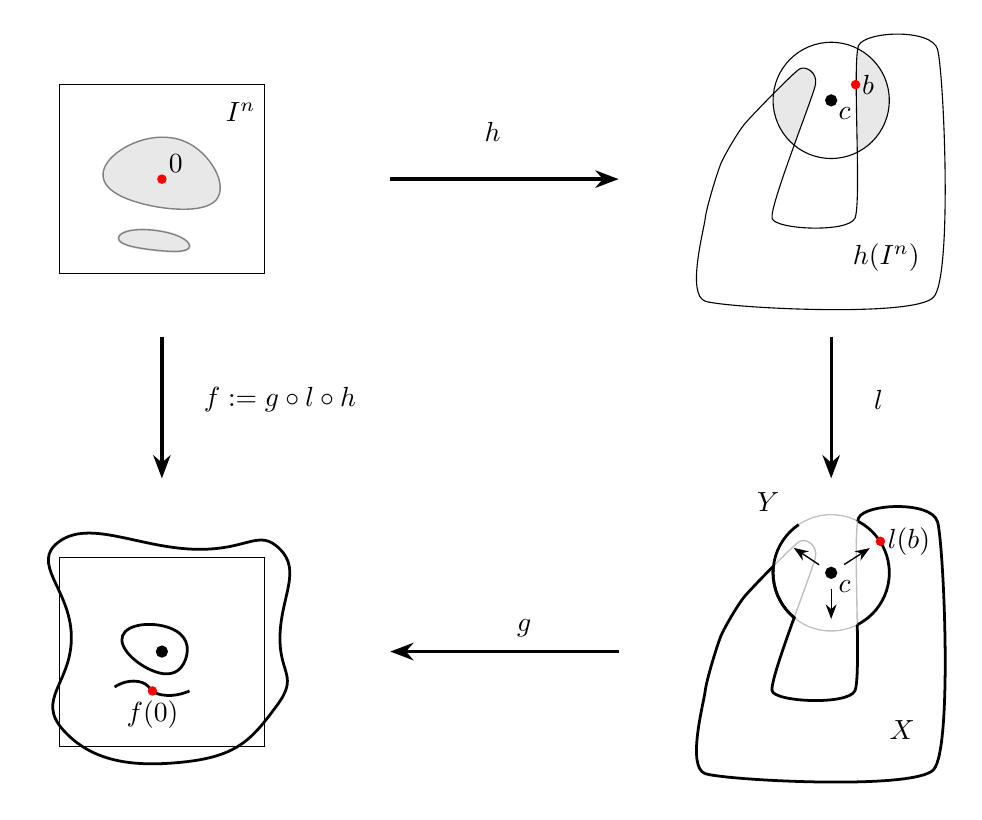
\begin{tikzpicture}
% ###############          prva slika          ###############
		\filldraw[color=gray!18] plot [smooth cycle, tension = 0.9] coordinates {(-5.15, 3.35) (-5.15, 2.8) (-3.95, 2.7) (-4.25, 3.45)};
		\draw[gray, line width=0.5pt] plot [smooth cycle, tension = 0.9] coordinates {(-5.15, 3.35) (-5.15, 2.8) (-3.95, 2.7) (-4.25, 3.45)};
		\filldraw[color=gray!18, line width=1pt] plot [smooth cycle, tension = 1.1] coordinates {(-4.25, 2.15) (-4.7, 2.35) (-5.15, 2.25) (-4.7, 2.1)};
		\draw[gray, line width=0.5pt] plot [smooth cycle, tension = 1.1] coordinates {(-4.25, 2.15) (-4.7, 2.35) (-5.15, 2.25) (-4.7, 2.1)};
		\draw (-5.9, 1.8) rectangle (-3.3, 4.2);
		\filldraw[red] (-4.6, 3) circle (1.5pt) node[black, above right=-0.5mm] {$0$};
		\draw (-4.2, 3.1) ;	
		 \draw (-3.6, 3.85) node {$I^n$};
		
% ###############          druga slika          ###############
		\begin{scope}
			\clip plot [smooth cycle, tension = 0.3] coordinates {(2.3, 1.45) (5.2, 1.5) (5.25, 4.65) (4.25, 4.7) (4.2, 2.5) (3.15, 2.5) (3.7, 4.2) (3.5, 4.4) (2.8,3.7)  (2.5, 3.2) (2.3, 2.5)};
			\clip (3.9, 4) circle (21pt);
			\fill[color=gray!18] (-2,1.5) rectangle (6,5);
		\end{scope}
		\draw plot [smooth cycle, tension = 0.3] coordinates {(2.3, 1.45) (5.2, 1.5) (5.25, 4.65) (4.25, 4.7) (4.2, 2.5) (3.15, 2.5) (3.7, 4.2) (3.5, 4.4) (2.8,3.7)  (2.5, 3.2) (2.3, 2.5)};
		\filldraw[black] (3.9, 4) circle (2pt) node[black, below right=-0.4mm]{$c$};
		\filldraw[red] (4.21, 4.2) circle (1.5pt) node[black, right=-0.4mm] {$b$};
		\draw[black] (3.9, 4) circle (21pt);
		\draw (4.6, 2) node {$h(I^n)$};
	
% ###############          tretja slika          ###############
		\draw[lightgray, line width=0.5pt] (3.9, -2) circle (21pt);
		\draw[black, line width=1pt] plot [smooth cycle, tension = 0.3] coordinates {(2.3, -4.55) (5.2, -4.5) (5.25, -1.35) (4.25, -1.3) (4.2, -3.5) (3.15, -3.5) (3.7, -1.8) (3.5, -1.6) (2.8, -2.3)  (2.5, -2.8) (2.3, -3.5)};
		\filldraw[white] (3.9, -2) circle (20.5pt);
		\begin{scope}
			\clip (3.9, -2) circle (21pt);
			\draw[lightgray, line width=0.5pt] plot [smooth cycle, tension = 0.3] coordinates {(2.3, -4.55) (5.2, -4.5) (5.25, -1.35) (4.25, -1.3) (4.2, -3.5) (3.15, -3.5) (3.7, -1.8) (3.5, -1.6) (2.8, -2.3)  (2.5, -2.8) (2.3, -3.5)};
		\end{scope}
		\begin{scope}
			\clip (3.9, -2) -- (3.4, -1.26) -- (2.5, -1) -- (3.35, -2.7) -- cycle;
			\draw[black, line width=1pt] (3.9, -2) circle (21pt);
		\end{scope}
		\begin{scope}
			\clip plot [smooth cycle, tension = 0.3] coordinates {(2.3, -4.55) (5.2, -4.5) (5.25, -1.35) (4.25, -1.3) (4.2, -3.5) (3.15, -3.5) (3.7, -1.8) (3.5, -1.6) (2.8, -2.3)  (2.5, -2.8) (2.3, -3.5)};
			\draw[black, line width=1pt] (3.9, -2) circle (21pt);
		\end{scope}
		\filldraw[black] (3.9, -2) circle (2pt) node[black, below right=-0.4mm]{$c$};
		\draw[black, line width=0.5pt, -Stealth] ($($(3.9, -2)!.5!(4.525, -1.6)$)!5pt!(3.9, -2)$) --  ($($(3.9, -2)!.5!(4.525, -1.6)$)!6pt!(4.525, -1.6)$);
		\draw[black, line width=0.5pt, -Stealth] ($($(3.9, -2)!.5!((3.9, -2.75)$)!5pt!(3.9, -2)$) --  ($($(3.9, -2)!.5!((3.9, -2.75)$)!6pt!((3.9, -2.75)$);
		\draw[black, line width=0.5pt, -Stealth] ($($(3.9, -2)!.5!(3.3, -1.6)$)!5pt!(3.9, -2)$) --  ($($(3.9, -2)!.5!(3.3, -1.6)$)!6pt!(3.3, -1.6)$);
		\filldraw[red] (4.525, -1.6) circle (1.5pt) node[black, right=-0.3mm] {$l(b)$};
		\draw (3.1, -1.1) node {$Y$};
		\draw (4.8, -4) node {$X$}; 
		
	% ###############          četrta slika          ###############
		\draw (-5.9, -4.2) rectangle (-3.3, -1.8);
		\draw[black, line width=1pt] plot [smooth cycle, tension = 1] coordinates {(-4.5, -2.7) (-4.3, -3.1) (-4.7, -3.25) (-5.1, -2.8)};
		\draw[black, line width=1pt] plot [smooth, tension = 1] coordinates {(-5.2, -3.45) (-4.9, -3.38) (-4.6, -3.55) (-4.25, -3.5)};
		\filldraw[red] (-4.72, -3.5) circle (1.5pt) node[black, below] {$f(0)$};
		\filldraw[black] (-4.6, -3) circle (2pt);
		\draw[black, line width=1pt] plot [smooth cycle, tension = 0.9] coordinates { (-3.1, -1.7) (-4.2, -1.7) (-5.9, -1.6) (-5.75, -2.8) (-5.85, -4) (-4.3, -4.4) (-3.15, -3.7) (-3.1, -2.8)};
	
	% ###############          puščice          ###############
		\draw [black, line width=1.2pt, -Stealth] (-1.7,3) -- (1.2,3);
		\draw (-0.4, 3.6) node {$h$};
		\draw [black,  line width=1.2pt, -Stealth] (1.2, -3) -- (-1.7, -3);
		\draw (0, -2.7) node {$g$};
		\draw [black,  line width=1.2pt, -Stealth] (-4.6, 1) -- (-4.6, -0.8);
		\draw (-3.1, 0.2) node {$f  := g \circ l \circ h$};
		\draw [black,  line width=1.2pt, -Stealth] (3.9, 1) -- (3.9, -0.8);
		\draw (4.5, 0.2) node {$l$};  
	\end{tikzpicture}
	
\end{document}